\section{Migrationskonzepte}
\label{section_migrationskonzepte}
Die Ziele einer Migration sind in der Regel betriebswirtschaftlicher oder strategischer Natur. Im Rahmen des hier untersuchten Rahmengebietes einer kleinen Hochschule ist die Migration hin zu einem ganzheitlichen Informationsmanagement eine strategische Entscheidung. Diese Entscheidung beinhaltet einen verbesserten Anwendernutzen, eine Erweiterung des Funktionsumfanges, bessere Integration und Verzahnung verschiedener Softwaresysteme sowie möglichst einer Erhöhung der Produktivität bei möglichst verringerten Kosten. Zur Erstellung des Migrationskonzeptes bedarf es der Betrachtung der Kriterien für eine erfolgreiche Migration und der möglichen Migrationsstrategien.

\subsection{Kriterien für eine erfolgreiche Migration}
Im Rahmen der Migrationsplanung werden die verschiedenen Phasen der Migration geplant. Im Rahmen der Betrachtung einer kleinen Hochschule wurden in der gesamten Ausarbeitung beispielsweise die Ist-Analyse vorgenommen und eine Soll-Konzeption erstellt.

\begin{figure}[h!]
	\centering
	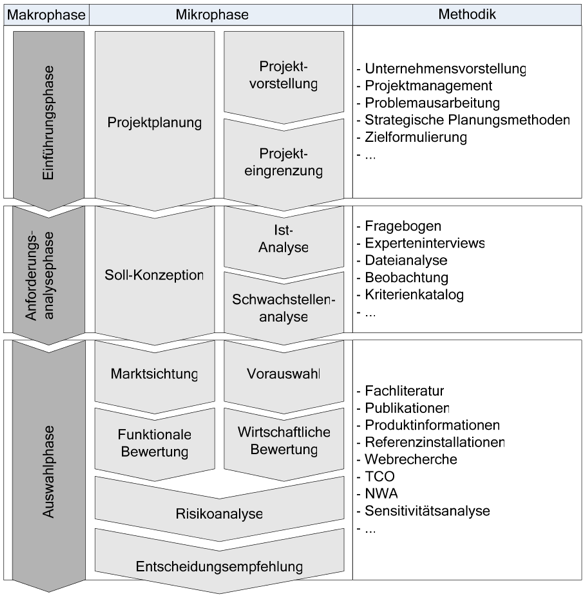
\includegraphics[width=10cm]{kapitel/gruppe4_1/bilder/vorgehensmodell_softwaremigration}
	\caption{Vorgehensmodell für Software-Migrationen nach \cite{migrationsleitfaden_2012}}
	\label{fig_vorgehensmodell_softwaremigration}	
\end{figure}

Das in Abbildung \ref{fig_vorgehensmodell_softwaremigration} ersichtliche Vorgehensmodell beschreibt die verschiedenen, notwendigen Phasen, die einer Migration vorausgehen. Die Genauigkeit dieser Planung ist hierbei maßgeblich für den späteren Erfolg der Migration. Im Rahmen dieser Ausarbeitung wurde beispielsweise die in der Abbildung ersichtliche Methodik des Experteninterviews angewandt, um Grundlagen für die Ist-Analyse zu erhalten.

In der Auswahlphase sind hierbei strategische, rechtliche und wirtschaftliche Aspekte zu berücksichtigen, ebenso wie der spätere Systembetrieb, die notwendigen organisatorischen Aspekte und Anforderungen an die Sicherheit der Systeme. Nach der Entscheidungsempfehlung werden dann eine oder mehrere Migrationsstrategien für die Einführung der neuen und die Ablösung der alten Software festgelegt.

\subsection{Migrationsstrategien}
Die Wahl der Migrationsstrategie ist jeweils fallbezogen zu prüfen. Es ist auch denkbar, für verschiedene Systeme verschiedene Strategien zu nutzen. Nachfolgend werden auszugweise durch Prof. Dr. Markus Nüttgens\footnote{\url{http://www.enzyklopaedie-der-wirtschaftsinformatik.de/wi-enzyklopaedie/lexikon/is-management/Integration-und-Migration-von-IT-Systemen/Ablosung-von-Altsystemen}} beschriebene Migrationsstrategien aufgeführt, welche in Abschnitt \ref{subsection_migrationsbeispiele} hinsichtlich der Verwendung durch die Migrationsbeispiele der Hochschule beleuchtet werden.

\begin{itemize}
	\item \textbf{Big Bang Approach (Cold Turkey Strategy):} Hierbei wird das Altsystem von Grund auf neu entwickelt und zu einem bestimmten Zeitpunkt zur Verfügung gestellt.	
	
	\item \textbf{Database First Approach / Database Last Approach:} Bei dieser Strategie wird erst das Datenbankmanagementsystem (Database First) migriert und anschließend alle Applikationen und Schnittstellen in ein neues System überführt. Database Last beschreibt hierbei den genau umgekehrten Vorgang.
	
	\item \textbf{Composite Database Approach:} Das neue Anwendungssystem wird schrittweise implementiert, während das Altsystem noch in Betrieb ist.
	
	\item \textbf{Chicken-Little Strategy:} Als Erweiterung des Composite Datebase Approach werden im Rahmen dieser Strategie zusätzliche Gateways entwickelt, welche für die Überführung der Daten aus dem Altsystem in das Zielsystem verantwortlich zeichnen.
	
	\item \textbf{Butterfly Methodology:} Hierbei geht es um eine reine Datenmigration, bei der eine Kooperation zwischen Alt- und Neusystem nicht notwendig ist.  Die Entwicklung des neuen Systems wird also von der Migration der Daten separiert.
\end{itemize}


\subsection{Migrationsbeispiele}
\label{subsection_migrationsbeispiele}

Die Hochschule Emden/Leer nutzt derzeit für Ihren Internetauftritt das Enterprise Content Management System TYPO3 in der Version 4.5. Die Dokumentenverwaltungssoftware Alfresco wird derzeit noch nicht genutzt. 

Die folgenden Beispiele behandeln eine mögliche Migration von TYPO3 auf eine aktuelle Version inkl. Erstellung eines responsive Designs, sowie die Neueinführung von Alfresco. Da die aktuelle Version von Alfresco auch die Möglichkeit bietet Web Content zu verwalten, wäre theoretisch auch eine Migration des derzeitigen Internetauftritts in ein neu eingeführtes Alfresco-System denkbar.

\subsubsection{Responsive Website mit TYPO3}
TYPO3\footnote{\url{http://typo3.org/typo3-cms/overview/}, abgerufen am 28.05.2015} ist ein Open Source Enterprise Content Management System zur Verwaltung webbasierter Inhalte. Es ist multilingual, hoch skalierbar und bietet ein aktives Sicherheitsmanagement.

\paragraph{Ist-Zustand}
Die Hochschule Emden/Leer nutzt derzeit ein TYPO3-Sytem in der Version 4.5 LTS (Long Term Support). Das System ist derzeit noch nicht für die Anforderungen mobiler Endgeräte (responsive Design) gerüstet. Es werden verschiedene Extensions von TYPO3 genutzt, möglicherweise auch eigens für die Hochschule entwickelte Extensions. Mitarbeiter und Studenten sind als Benutzer innerhalb des CMS angelegt und können sich in einen geschützten Bereich über die Extension FE-Login anmelden.

Für die derzeit eingesetzte Version von TYPO3 gibt es keinen Support mehr, so dass – weder für den TYPO3-Kern, noch für die Extensions – neue Sicherheitspatches zur Verfügung gestellt werden. Dies stellt ein Sicherheitsrisiko für die Hochschule dar. Allein aus diesem Grund sollte eine Migration auf ein aktuelles System erwogen werden. Ferner nutzt ein Großteil der Besucher mobile Endgeräte, die aktuell nicht unterstützt werden.

\paragraph{Soll-Zustand}\mbox{}\\
Das neue System soll über folgende Merkmale verfügen:
\begin{itemize}
\item lange Support-Zeit, damit Sicherheitspatches eingespielt werden können
\item Unterstützung von mobilen Endgeräten
\item Übernahme bestehender Extensions oder Vorhandensein von Alternativen hierzu
\item Barrierefreiheit, damit auch Benutzer mit Handicap den Internetauftritt besuchen können
\item Suchmaschinenoptimierung (SEO)
\item Anbindung an die Benutzerverwaltung (Single-Sign-On) der Hochschule (bereits realisiert)
\end{itemize}
Hierzu wird zunächst ein strategisch günstiger Migrationsplan erstellt.

\paragraph{Migrationsplan}\mbox{}\\
Um einen möglichst langen Supportzeitraum zu gewährleisten ist die Verwendung einer LTS-Version (Long Term Support) anzuraten. Die derzeit aktuelle Version ist 6.2.12 LTS (Stand 27.05.2015), welche noch bis Ende März 2017 supportet wird.

Derzeit ist bereits die Version 7.2.0 verfügbar, allerdings noch nicht als LTS-Version. Diese ist für Herbst 2015 avisiert. 

Da die Migration einige Zeit in Anspruch nehmen wird, ist es sinnvoll, direkt auf die Version 7.x LTS zu migrieren, da diese dann verfügbar sein wird. Hierfür sind allerdings Zwischenschritte vorzusehen, da eine direkte Migration von Version 4.5 auf 7.x nicht möglich ist.\footnote{\url{http://wiki.typo3.org/Upgrade}, abgerufen am 28.05.2015} Es muss zunächst eine Migration auf die Version 6.2 LTS und von dort auf die Version 7.x erfolgen. Nachfolgend wird somit von einer Migration auf die Version 7.x LTS ausgegangen.

Vor der Migration ist eine Überprüfung aller derzeit genutzten Extensions erforderlich. Dabei muss geprüft werden, ob diese in der neuen Version noch gültig und lauffähig sind. Ist dies nicht der Fall, müssen Alternativen gesucht werden und deren Realisierung in die Planung einfließen. Insbesondere selbst geschriebene Extensions müssen hinsichtlich der Lauffähigkeit überprüft und ggf. ein Konzept zur Anpassung erstellt werden.

\subparagraph{Hardwareanforderungen}\mbox{}\\
Für eine erfolgreiche Migration sind bestimmte Hardwareanforderungen Voraussetzung. Unter anderem muss mindestens PHP 5.5, MySQL 5.5 und mehr als 200 MB freier Plattenplatz zur Verfügung stehen. Die genauen Konfigurationseinstellungen inkl. allen benötigten Module sind den Installationsvorgaben der TYPO3 Association zu entnehmen.

\subparagraph{Entwicklungssystem}\mbox{}\\
Zur Realisierung des neuen Systems wird ein Entwicklungssystem mit den oben beschriebenen Hardwareanforderungen aufgesetzt. Über einen Dump der Datenbank werden die Daten des Produkivsystems in die Datenbank des Entwicklungssystems übertragen. Das gesamte Dateisystem des TYPO3-Produktivsystems wird ebenfalls auf das Entwicklungssystem übertragen. Dort werden dann die Konfigurationseinstellungen von TYPO3 angepasst, damit ein identisches, lauffähiges System entsteht.

Innerhalb dieses Systems erfolgt die Migration auf die verschiedenen Versionen, die Anpassung der Extensions und die im Rahmen der Migration notwendige Softwareentwicklung.

\subparagraph{Migration}\mbox{}\\
Im Rahmen der Migration müssen Softwaretechnisch folgende Punkte berücksichtigt werden:
\begin{itemize}
\item Migration des TYPO3-Kerns
\item Migration aller eingesetzten Extensions
\item Anpassung selbstgeschriebener Extensions
\item Umstellung des Layout-Konzeptes von TYPO3 (von derzeit wahrscheinlich Templa-Voilà) auf Fluid-Templating
\item Schaffung einer Basis für responsive Design, beispielsweise auf Basis des Frameworks Bootstrap
\item Erweiterung / Anpassung der TypoScript-Programmierung
\item Anpassung Menüprogrammierung (TypoScript und Template)
\item Neuerstellung benötigter Fluid-Templates auf Basis von Haupttemplates und Partials
\item Programmierung eigener Extensions, falls notwendig
\end{itemize}

\subparagraph{Produktivsetzung}\mbox{}\\
Die Ablösung des derzeitigen Systems erfolgt anhand der Migrationsstrategie Big Bang Approach, da mit dem Entwicklungssystem ein fertig entwickeltes und hinsichtlich des Datenbestandes aktuelles System zur Verfügung steht. Die Produktivsetzung erfolgt in umgekehrter Reihenfolge wie die Einrichtung des Entwicklungssystems, also mit Datenbank-Dump, Datei-Migration und ggf. TYPO3-Konfigurations-anpassungen. Hierdurch ist die Downtime für den Internetauftritt der Hochschule Emden minimal.

\subsubsection{Alfresco}
Alfresco\footnote{\url{https://www.alfresco.com/de/solutions/document-management}, abgerufen am 28.05.2015} ist ein Dokumenten-Management-System welches als Open-Source-Plattform offene Standards unterstützt. Hiermit lässt sich der gesamte Content auf einer einzelnen Plattform konsolidieren und damit die Benutzerfreundlichkeit erhöhen und die Kosten senken.

Luis Cabaceira\footnote{\url{http://de.slideshare.net/LuisCabaceira/sizing-your-alfrescoplatform}, abgerufen am 27.05.2015} hat die nachfolgende Grafik erstellt, die eine Übersicht über die Funktionen von Alfresco gibt:

\begin{figure}[h!]
	\centering
	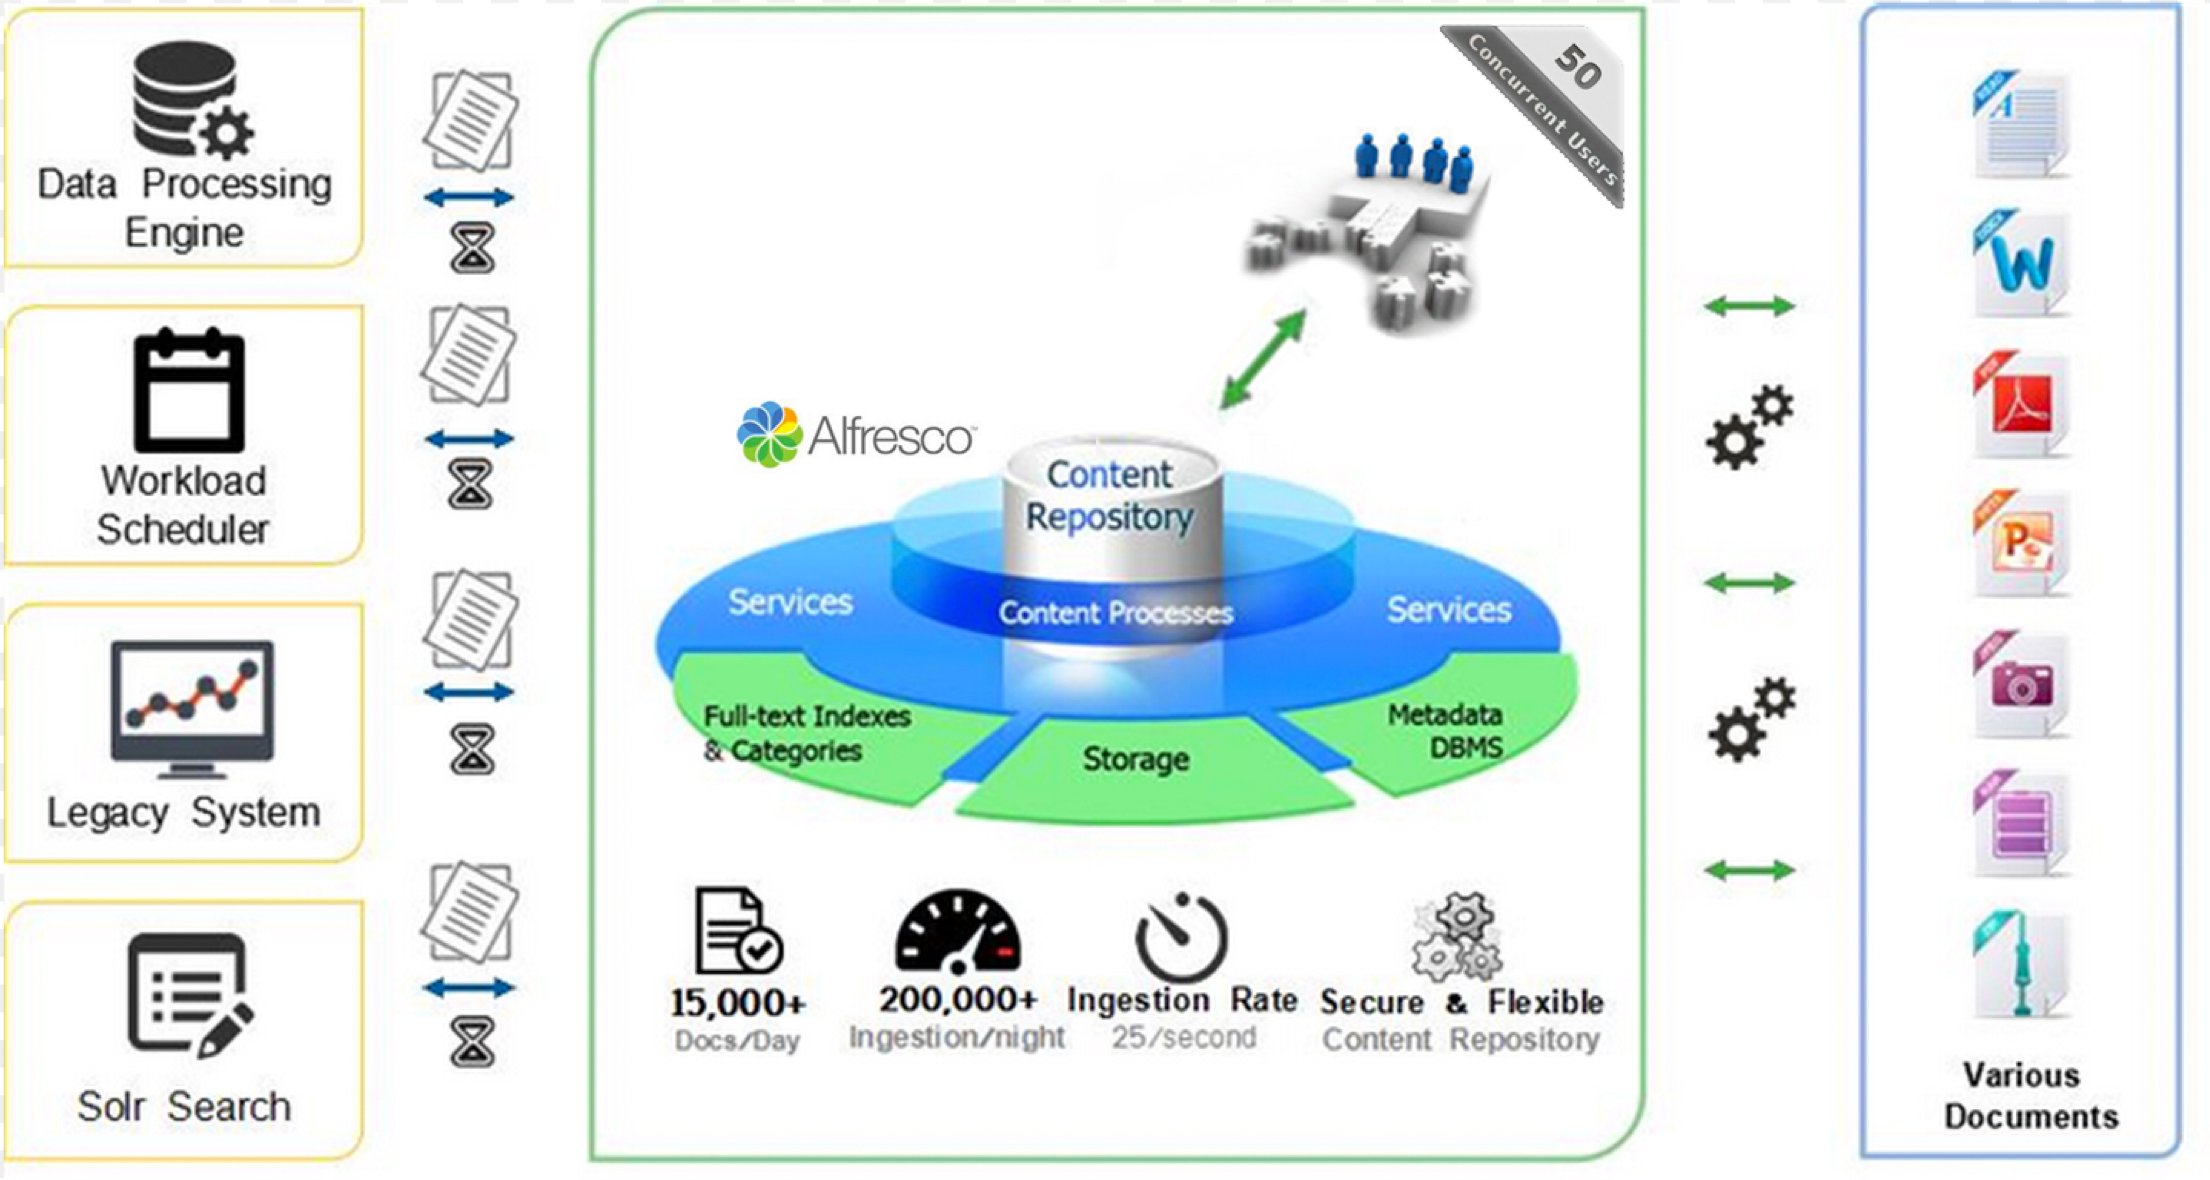
\includegraphics[width=10cm]{kapitel/gruppe4_1/bilder/uebersicht_alfresco}
	\caption{Übersicht Alfresco nach Luis Cabaceira}
	\label{fig_uebersicht_alfresco}
\end{figure}

Peter Franke – Leiter des Rechenzentrums der Hochschule Braunschweig/Wolfenbüttel – berichtet von positiven Erfahrungen seit der Einführung von Alfresco.\footnote{\url{http://www.ostfalia.de/export/sites/default/de/rz/documents/it-konzept-2011.pdf}, abgerufen am 27.05.2015}

\paragraph{Ist-Zustand}
Alfresco wird derzeit von der Hochschule Emden/Leer noch nicht eingesetzt. Derzeit werden Dokumente in verschiedensten Systemen verwaltet und zugänglich gemacht. Auszugsweise sind hier zu nennen:

\begin{itemize}
	\item Austauschlaufwerke für Dozenten
	\item Webseiten mit offenen und geschlossenen Bereichen (Kennzahlen, Daten, Fakten für Mitarbeiter und Dekane)
	\item Eigene Software Vorlesungsverzeichnis im Fachbereich Seefahrt
	\item Software EvaSys für die Evaluierung
	\item Gigamove zum Austausch große Datenmengen
	\item Eigene Systeme in den Fachbereichen (Labor)	
\end{itemize}

Derzeit gibt es also viele gewachsene Systeme und Strukturen.

\paragraph{Soll-Zustand}
Das neue System soll über folgende Merkmale verfügen:
\begin{itemize}
	\item Migration aller vorhandener Dokumente auf das neue System für eine zentrale Verwaltung
	\item Versionsmanagement
	\item Schneller Zugriff
	\item Ortsunabhängiger Zugriff
	\item Verwaltung verschiedenster Dokumenttypen
	\item Keine Client-Installation notwendig
\end{itemize}

Die Software Alfresco bietet alle diese Merkmale. In der aktuellen Version wird auch die Auslieferung von Web-Content unterstützt, so dass für die Zukunft auch eine Migration des Internetauftritts in das Alfresco-System denkbar wäre. Alternativ könnte Alfresco auch im Rahmen des Single Source Publishing Konzeptes als Content-Quelle für das TYPO3-System genutzt werden. Die Berliner Philharmoniker nutzen bereits dieses Konzept, wie aus einer Case Study der Firma form4 GmbH hervorgeht.\footnote{\url{http://www.form4.de/artikel/alfresco-meets-typo3/}, abgerufen am 28.05.2015}

Hinsichtlich des Dokumenten-Managements wird zunächst ein strategisch günstiger Migrationsplan zur Einführung von Alfresco erstellt. Dabei muss auch die Entscheidung getroffen werden, welche Edition von Alfresco sinnvoll für die Hochschule ist.

\paragraph{Migrationsplan}
Da nach der Migration alle Dokumente zentral verwaltet werden, erscheint es sinnvoll, Alfresco als hochverfügbaren Cluster auszulegen. Gegebenenfalls ist auch der Einsatz eines SAN (Storage Area Networks) mit räumlich getrennten Speichereinheiten und entsprechend angepasstem Backup- und Restore-Konzept in Erwägung zu ziehen.

Grundsätzlich stehen von Alfresco die kostenlose Community Edition und die kostenpflichtige Enterprise Edition zur Verfügung. Ein Vergleich der beiden Editionen findet sich auf der Website\footnote{\url{https://www.alfresco.com/de/alfresco-community-edition}, abgerufen am 28.05.2015} von Alfresco.

\subparagraph{Hardwareanforderungen}
Die Hardwareanforderungen richten sich stark nach den in Alfresco genutzten Modulen, bzw. ob die Community oder Enterprise-Edition genutzt wird. Detailliert Hardwareanforderungen können nach Festlegung der Edition in der Alfresco-Dokumentation\footnote{\url{http://docs.alfresco.com/5.0/concepts/ha-intro.html}, abgerufen am 28.05.2015} eingesehen werden. 

Die Hardwareanforderungen sind unter anderem abhängig von:

\begin{itemize}
	\item dem benötigten Anwendungsfall (welche Komponenten genutzt werden)
	\item der Anzahl der gleichzeitig zugreifenden Benutzer
	\item dem Speicherort der Dokumente
	\item dem Betrieb im Rahmen einer Hochverfügbarkeitslösung
	\item dem Einsatz von Load Balancern
	\item dem Einsatz dedizierter Transformation Server
	\item der Nutzung von Clustern für zu nutzende Interfaces
	\item dem Einsatz von Caching-Verfahren
\end{itemize}

\begin{figure}[h!]
	\centering
	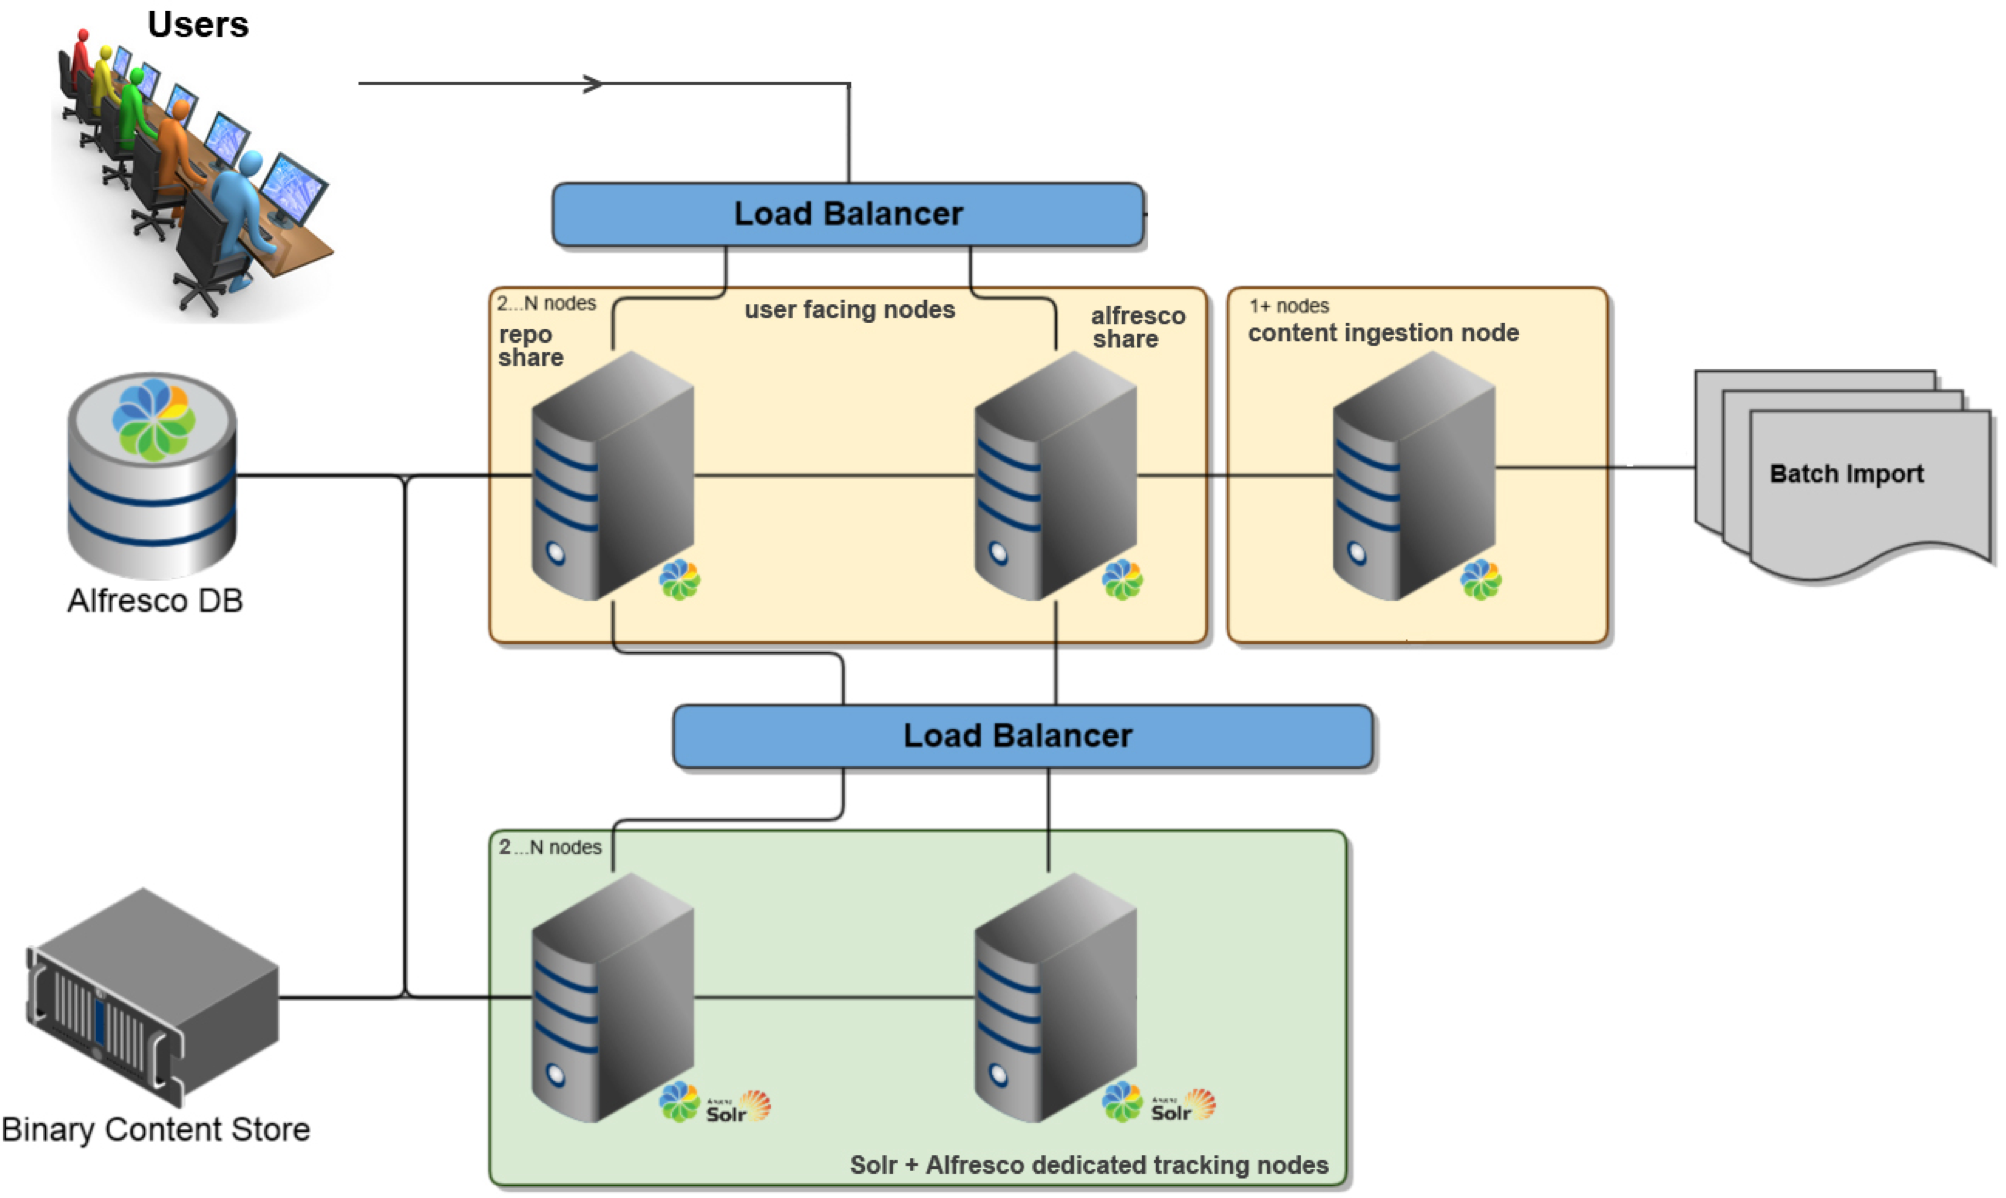
\includegraphics[width=10cm]{kapitel/gruppe4_1/bilder/deployment_diagramm_alfresco}
	\caption{Mögliche Hardwarestruktur für Alfresco nach Cabaceira, 2014}
	\label{fig_deployment_alfresco}
\end{figure}

Die Abbildung \ref{fig_deployment_alfresco} zeigt eine mögliche Hardwarestruktur für ein Alfresco-System nach Cabaceira.\footnote{\url{http://de.slideshare.net/LuisCabaceira/sizing-your-alfrescoplatform}, abgerufen am 27.05.2015}

\subparagraph{Entwicklungssystem}
Das Entwicklungssystem wird nach den benötigten Hardwareanforderungen aufgesetzt. Hierauf erfolgt die Implementierung von Alfresco inkl. den bei Bedarf benötigten Schnittstellen. Nach Fertigstellung kann das Entwicklungssystems direkt als Produktivsystem genutzt werden, da die Datenmigration anschließend erfolgt, wie im folgenden Abschnitt beschrieben.

\subparagraph{Migration}
Für die Migration bietet sich in diesem Fall die Migrationsstrategie Butterfly Methodology an, da hierbei nach und nach die verschiedenen Altsysteme in das neue System überführt werden können. Da es sich beim Entwicklungssystem um ein "leeres" System handelt, wird es nach Fertigstellung als Produktivsystem genutzt. Hierin erfolgt dann nach und nach die Migration der Dokumente aus den unterschiedlichen Altsystemen.

\subparagraph{Produktivsetzung}
Wie bereits oben beschrieben, erfolgt die Produktivsetzung direkt nach Abnahme des Entwicklungssystem und erfolgt durch dessen Übernahme.

